\section{Results}
The data of the ACAR experiment is shown in Figure \ref{fig:bg}. The shape of the curve is, as expected, a combination of a Gaussian, parabola and a convolution function, as was discussed in the previous chapters.\begin{figure}[H]
\centering
\resizebox{\columnwidth}{!}{% GNUPLOT: LaTeX picture with Postscript
\begingroup
  \makeatletter
  \providecommand\color[2][]{%
    \GenericError{(gnuplot) \space\space\space\@spaces}{%
      Package color not loaded in conjunction with
      terminal option `colourtext'%
    }{See the gnuplot documentation for explanation.%
    }{Either use 'blacktext' in gnuplot or load the package
      color.sty in LaTeX.}%
    \renewcommand\color[2][]{}%
  }%
  \providecommand\includegraphics[2][]{%
    \GenericError{(gnuplot) \space\space\space\@spaces}{%
      Package graphicx or graphics not loaded%
    }{See the gnuplot documentation for explanation.%
    }{The gnuplot epslatex terminal needs graphicx.sty or graphics.sty.}%
    \renewcommand\includegraphics[2][]{}%
  }%
  \providecommand\rotatebox[2]{#2}%
  \@ifundefined{ifGPcolor}{%
    \newif\ifGPcolor
    \GPcolortrue
  }{}%
  \@ifundefined{ifGPblacktext}{%
    \newif\ifGPblacktext
    \GPblacktextfalse
  }{}%
  % define a \g@addto@macro without @ in the name:
  \let\gplgaddtomacro\g@addto@macro
  % define empty templates for all commands taking text:
  \gdef\gplbacktext{}%
  \gdef\gplfronttext{}%
  \makeatother
  \ifGPblacktext
    % no textcolor at all
    \def\colorrgb#1{}%
    \def\colorgray#1{}%
  \else
    % gray or color?
    \ifGPcolor
      \def\colorrgb#1{\color[rgb]{#1}}%
      \def\colorgray#1{\color[gray]{#1}}%
      \expandafter\def\csname LTw\endcsname{\color{white}}%
      \expandafter\def\csname LTb\endcsname{\color{black}}%
      \expandafter\def\csname LTa\endcsname{\color{black}}%
      \expandafter\def\csname LT0\endcsname{\color[rgb]{1,0,0}}%
      \expandafter\def\csname LT1\endcsname{\color[rgb]{0,1,0}}%
      \expandafter\def\csname LT2\endcsname{\color[rgb]{0,0,1}}%
      \expandafter\def\csname LT3\endcsname{\color[rgb]{1,0,1}}%
      \expandafter\def\csname LT4\endcsname{\color[rgb]{0,1,1}}%
      \expandafter\def\csname LT5\endcsname{\color[rgb]{1,1,0}}%
      \expandafter\def\csname LT6\endcsname{\color[rgb]{0,0,0}}%
      \expandafter\def\csname LT7\endcsname{\color[rgb]{1,0.3,0}}%
      \expandafter\def\csname LT8\endcsname{\color[rgb]{0.5,0.5,0.5}}%
    \else
      % gray
      \def\colorrgb#1{\color{black}}%
      \def\colorgray#1{\color[gray]{#1}}%
      \expandafter\def\csname LTw\endcsname{\color{white}}%
      \expandafter\def\csname LTb\endcsname{\color{black}}%
      \expandafter\def\csname LTa\endcsname{\color{black}}%
      \expandafter\def\csname LT0\endcsname{\color{black}}%
      \expandafter\def\csname LT1\endcsname{\color{black}}%
      \expandafter\def\csname LT2\endcsname{\color{black}}%
      \expandafter\def\csname LT3\endcsname{\color{black}}%
      \expandafter\def\csname LT4\endcsname{\color{black}}%
      \expandafter\def\csname LT5\endcsname{\color{black}}%
      \expandafter\def\csname LT6\endcsname{\color{black}}%
      \expandafter\def\csname LT7\endcsname{\color{black}}%
      \expandafter\def\csname LT8\endcsname{\color{black}}%
    \fi
  \fi
  \setlength{\unitlength}{0.0500bp}%
  \begin{picture}(5668.00,3400.00)%
    \gplgaddtomacro\gplbacktext{%
      \csname LTb\endcsname%
      \put(860,640){\makebox(0,0)[r]{\strut{} 0}}%
      \csname LTb\endcsname%
      \put(860,955){\makebox(0,0)[r]{\strut{} 50}}%
      \csname LTb\endcsname%
      \put(860,1270){\makebox(0,0)[r]{\strut{} 100}}%
      \csname LTb\endcsname%
      \put(860,1585){\makebox(0,0)[r]{\strut{} 150}}%
      \csname LTb\endcsname%
      \put(860,1900){\makebox(0,0)[r]{\strut{} 200}}%
      \csname LTb\endcsname%
      \put(860,2214){\makebox(0,0)[r]{\strut{} 250}}%
      \csname LTb\endcsname%
      \put(860,2529){\makebox(0,0)[r]{\strut{} 300}}%
      \csname LTb\endcsname%
      \put(860,2844){\makebox(0,0)[r]{\strut{} 350}}%
      \csname LTb\endcsname%
      \put(860,3159){\makebox(0,0)[r]{\strut{} 400}}%
      \csname LTb\endcsname%
      \put(980,440){\makebox(0,0){\strut{}-2}}%
      \csname LTb\endcsname%
      \put(1521,440){\makebox(0,0){\strut{}-1.5}}%
      \csname LTb\endcsname%
      \put(2062,440){\makebox(0,0){\strut{}-1}}%
      \csname LTb\endcsname%
      \put(2603,440){\makebox(0,0){\strut{}-0.5}}%
      \csname LTb\endcsname%
      \put(3144,440){\makebox(0,0){\strut{} 0}}%
      \csname LTb\endcsname%
      \put(3684,440){\makebox(0,0){\strut{} 0.5}}%
      \csname LTb\endcsname%
      \put(4225,440){\makebox(0,0){\strut{} 1}}%
      \csname LTb\endcsname%
      \put(4766,440){\makebox(0,0){\strut{} 1.5}}%
      \csname LTb\endcsname%
      \put(5307,440){\makebox(0,0){\strut{} 2}}%
      \put(160,1899){\rotatebox{-270}{\makebox(0,0){\strut{}Counts}}}%
      \put(3143,140){\makebox(0,0){\strut{}Angle [	extdegree]}}%
    }%
    \gplgaddtomacro\gplfronttext{%
    }%
    \gplbacktext
    \put(0,0){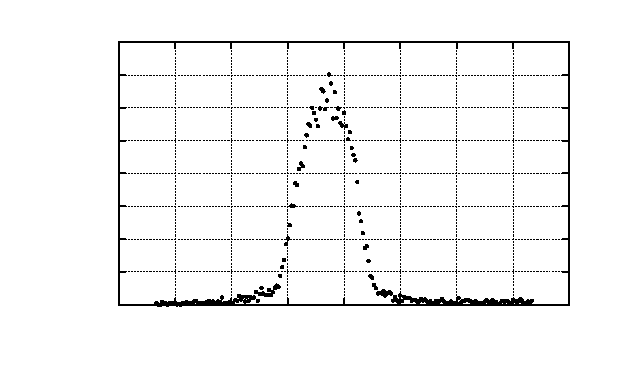
\includegraphics{bg}}%
    \gplfronttext
  \end{picture}%
\endgroup
}
\caption{Angle correlation between 511~keV annihilation photons. The angle was changed with an increment of 0.017~$^{\circ}$ and data was acquired for 2160~s per angle. q}
\label{fig:bg}
\end{figure} To obtain the parameters that best fit the measured data, a least squares method is performed in LabVIEW by calculating the sum of the squared residuals for each combination of the parameters over a suitable range. First the plausible ranges of values for the parameters were found by hand. Taking into account desired accuracy and program runtime (the program is $O(n)$), the stepsize and amount of steps for each parameter is selected accordingly. The following values were selected: \begin{table}[H]
    \begin{tabularx}{\linewidth}{X l l l}
    Parameter & Start value & Step size & Steps\\ \hline\hline
    Fermi angle $\theta_{F}$  & 6.65~mrad & 0.01 & 65\\
    Core width & 5.8~mrad & 0.01 & 20\\
    Fraction core annihilations & 0.15 & 0.05 & 8 \\
    Slitwidth& 0.5~mm & 0.05 & 20 \\
    $^{22}$Na source radius & 0.007~mm & 0.001 & 6 \\
    Background coincidence counts & 1 & 0.05 & 20\\
    Alignment correction & 1.6 & 0.01 & 250 \\ \hline
    \end{tabularx}
\end{table} The collimator distance was fixed to 600~mm. A minimum for the squared and summed residuals was found when the parameters were set to: \begin{table}[H]
    \begin{tabularx}{\linewidth}{l X}
    Parameter & Value\\ \hline\hline
    Fermi angle $\theta_{F}$ & 6.98~\text{mrad}\\
    Core width & 5.94 mrad\\
    Fraction core annihilations & 0.20 \\
    Slitwidth & 1.10 mm\\
    $^{22}$Na source radius & 0.01 mm\\
    Background coincidence counts & 1.45\\
    Alignment correction & 2.73 \\ \hline
    \end{tabularx}
\end{table} The Fermi energy corresponding to a Fermi angle of 6.98 milliradians equals 12.46~eV. The literature value for the Fermi energy of aluminium is 11.65~eV \cite{Massalski1978151, ashcroft1976solid}. This deviation from the literature value most likely originates from the fitting process. During manual fitting it was observed that small deviations in certain parameters had a significant effect on the value for the Fermi angle that produced the lowest squared and summed residuals. Another explanation would be the inaccuracies caused by the approximation that the positron is stationary during the electron-positron annihilation process. 